\TODO{still lacks better intros}
% problem intro
Currently an architect starts the building design work flow by drawing rough
free form sketches of the desired building. These drawings are highly subjective
and clients have a hard time in their interpretation and validation.
The information captured in such drawings has little use in the remaining stages
of building design.

\TODO{insert draft sketches}

There are systems which are commonly used for professional building layouts
such as Autodesk Autocad \cite{SITE-AUTOCAD}.
The architect replicates his former ideas in the rigid standardized interface
offered by these systems. This is a rigorous endeavor, taking much time to be asserted.

After the main project documents are issued comes the time when the idea has to
be pitched to end clients.
In order to gather buyers and investors its common to generate colorful previews of the building featuring increasingly realistic features such as detailed materials, light propagation and crowd simulations. See
Fig. \ref{FIG-REALISTIC}.

\begin{figure}[!ht]
	\centering
	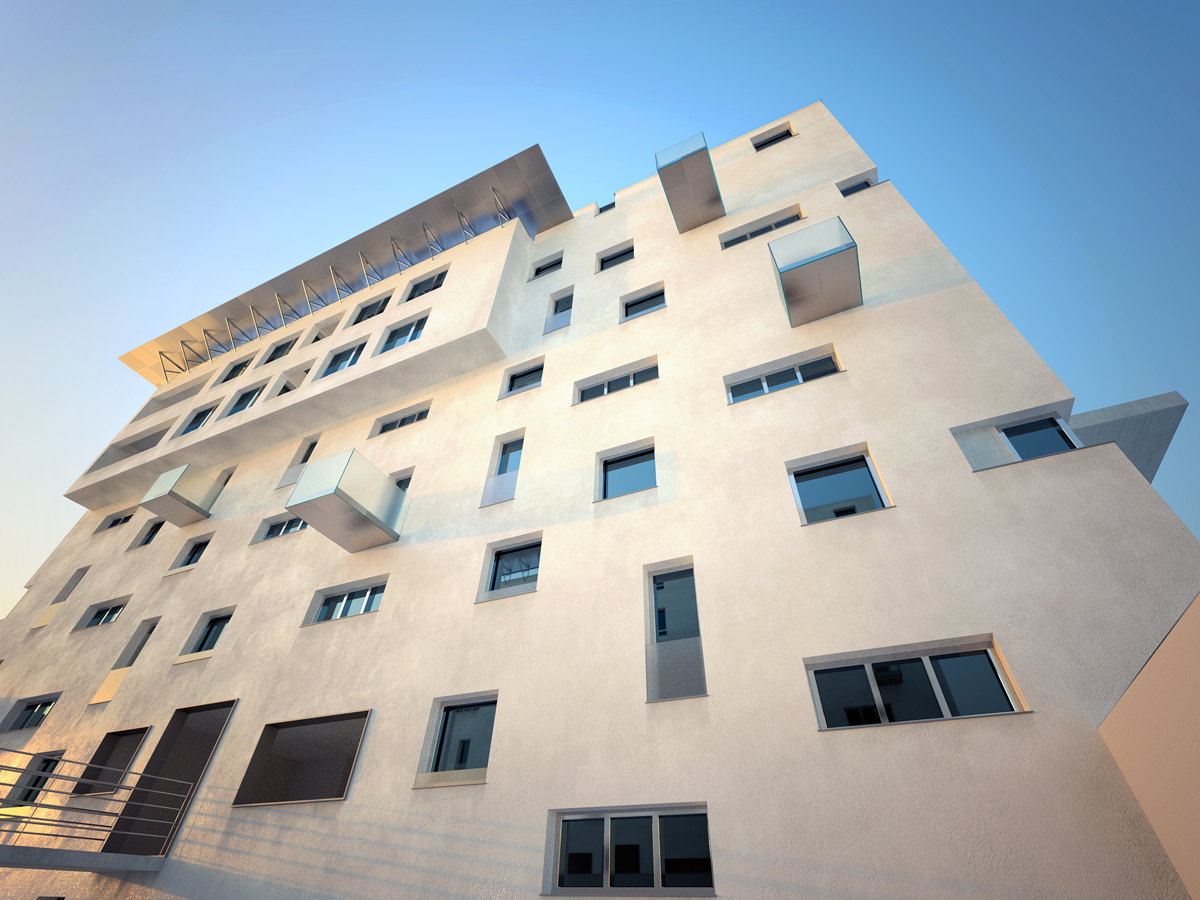
\includegraphics[width=6cm]{gfx/realistic01.jpg}
	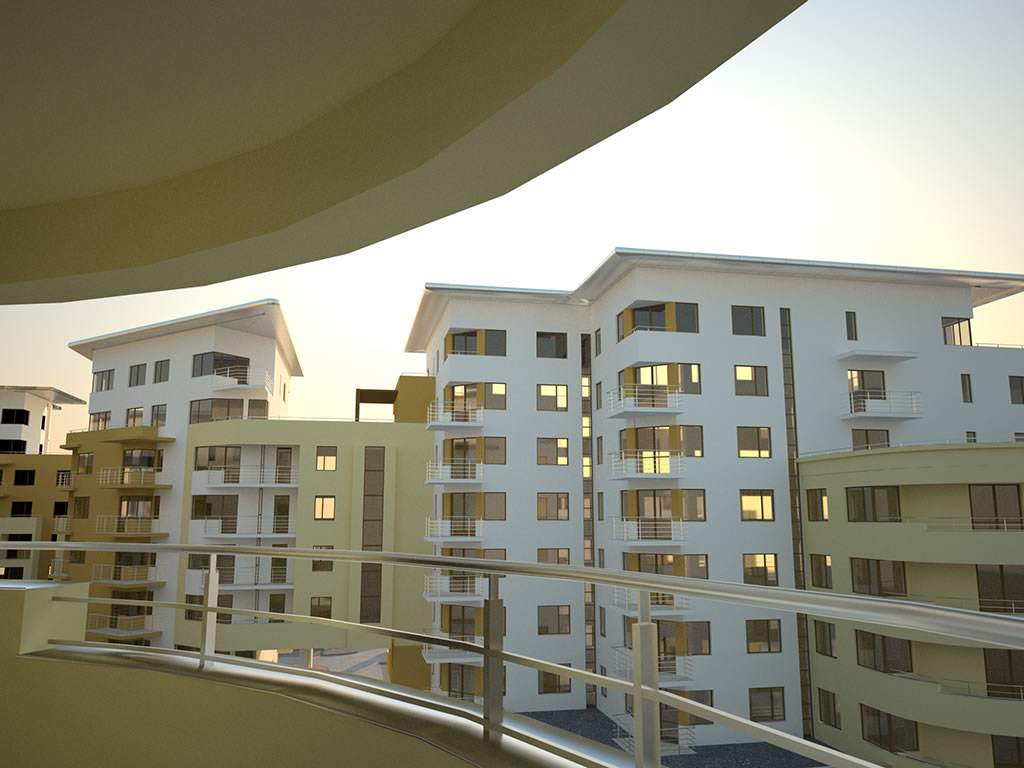
\includegraphics[width=6cm]{gfx/realistic03.jpg}
	\caption{Realistic renderings done with Maxwell Renderer}
	\label{FIG-REALISTIC}
\end{figure}

Despite the advances in computation, the architect work flow keeps these three separated stages
that don't share media or applications (Fig. \ref{FIG-WORKFLOW1}).
Both the conceptual design stage and the final reviewing and marketing stage would benefit from 
an integrated system with a comprehensive set of design actions and good navigation and annotation
capabilities.

\begin{figure}[!ht]
	\centering
	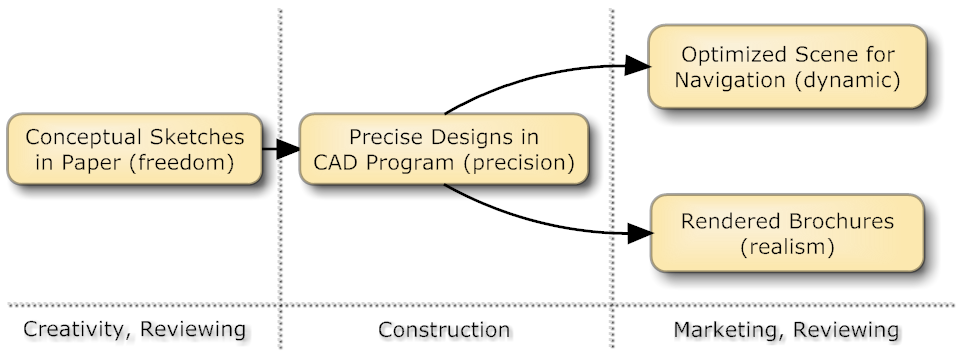
\includegraphics[width=12cm]{gfx/workflow1.png}
	\caption{Architect's project work flow}
	\label{FIG-WORKFLOW1}
\end{figure}

In order for an architect to use a computer program for drawing early designs,
it must be flexible enough not to limit the architect in expressing his vision.
Most current systems constrain architect's creativity \cite{TOW3D}.

% beautification
Sketching beautification supports this feature by interpreting strokes
into lines and other geometric primitives.

% 2D->3D
There are commonly drawn shapes in architecture such as box shaped walls or windows.
The enhanced strokes shall then be interpreted to generate 3D shapes such as these.

% suggestive
The system might also identify geometry constraints such as parallelism and symmetry,
suggesting the designer with precise alternatives for his strokes.

% multimodal int.
A set of input and output devices must then be assembled with the purpose of offering
the users an immersive experience. Therefore this set must be chosen and
means must be given to users to allow them to perform actions like walking or creating
annotations.

% navigation, multi user
Having also the purpose of client reviewing and showcasing of designs,
the system should offer a comprehensive interface,
one that aids the user in navigating the world with a gentle learning curve.
Reviewing could also be done remotely.
Either in a local or remote set, the system should allow
concurrent browsing and editing of the world.

% knowledge rep.
A building can be as detailed as we want it to be.
The system must be robust and enough to represent a city block, therefore it must have a
robust representation of buildings and other structures composing the world.

